\documentclass[11pt]{article}

% ---------------------------------------------------------------------------
%  Parallelising timed-automata reachability: OpenMP and Metal GPU backends
% ---------------------------------------------------------------------------
\usepackage[utf8]{inputenc}
\usepackage[T1]{fontenc}
\usepackage{lmodern}
\usepackage[a4paper,margin=2.4cm]{geometry}
\usepackage{amsmath,amssymb,amsthm}
\usepackage{booktabs}
\usepackage{xcolor}
\usepackage{graphicx}
\usepackage{caption}
\usepackage{subcaption}
\usepackage{algorithm}
\usepackage{algpseudocode}
\usepackage{listings}
\usepackage{microtype}
\usepackage{tikz}
\usepackage{pgfplots}
\pgfplotsset{compat=1.18}
\usetikzlibrary{arrows.meta,positioning,calc,fit,backgrounds,shapes.geometric,
                decorations.pathreplacing,shadows.blur,matrix}
\usepackage[hidelinks]{hyperref}
\usepackage[nameinlink]{cleveref}

% ---- palette --------------------------------------------------------------
\definecolor{cpu}{HTML}{2C6E9B}     % blue   -- host / CPU
\definecolor{gpu}{HTML}{B5651D}     % orange -- GPU
\definecolor{acc}{HTML}{3F7A3F}     % green  -- accents
\definecolor{soft}{HTML}{F1F4F8}
\definecolor{softg}{HTML}{FBEFE3}
\definecolor{codebg}{HTML}{F7F7F4}

% ---- tikz styles ----------------------------------------------------------
\tikzset{
  box/.style   ={rounded corners=2pt, draw=black!55, thick, align=center,
                 font=\small, inner sep=5pt, minimum height=8mm},
  cpubox/.style={box, fill=soft,  draw=cpu!70},
  gpubox/.style={box, fill=softg, draw=gpu!75},
  lane/.style  ={rounded corners=3pt, draw=black!25, thick, inner sep=7pt},
  flow/.style  ={-{Stealth[length=2.4mm]}, thick, draw=black!65},
  dflow/.style ={-{Stealth[length=2.4mm]}, thick, draw=black!45, dashed},
  lbl/.style   ={font=\scriptsize\itshape, text=black!60},
}

% ---- listings -------------------------------------------------------------
\lstset{
  basicstyle=\ttfamily\footnotesize, backgroundcolor=\color{codebg},
  breaklines=true, columns=fullflexible, keepspaces=true, frame=single,
  rulecolor=\color{black!20}, framesep=4pt, xleftmargin=4pt,
  commentstyle=\color{acc}, keywordstyle=\color{cpu}\bfseries,
  language=C++, showstringspaces=false, morekeywords={kernel,device,__global__,constant,thread}
}

\newtheorem{proposition}{Proposition}
\newcommand{\dk}{\ensuremath{\mathit{dk}}}
\newcommand{\aluleq}{\ensuremath{\preceq_{\mathrm{aLU}}}}
\newcommand{\code}[1]{\texttt{\small #1}}

\title{\bfseries Parallelising Timed-Automata Reachability:\\[2pt]
  \large A Shared-Memory (OpenMP) and a GPU (Metal/CUDA) Backend for a Timed-CTL Model Checker}
\author{PTCTLMC Project}
\date{\today}


% ---- extra packages used by this paper ------------------------------------
\usepackage{multirow}
\usetikzlibrary{patterns}

% ---- aliases: keep local figure code readable while using the house palette -
\colorlet{cA}{cpu}
\colorlet{cB}{gpu}
\colorlet{cC}{acc}
\colorlet{cD}{cpu!60!black}
\definecolor{cGrey}{HTML}{7F8C8D}

% ---- macros ---------------------------------------------------------------
\providecommand{\clockSet}{\mathcal{C}}
\providecommand{\Zone}{\mathcal{Z}}
\providecommand{\DBM}[1]{\mathbf{D}_{#1}}
\providecommand{\Passed}{\mathit{Passed}}
\providecommand{\dk}{\mathit{dk}}
\providecommand{\aLU}{\ensuremath{\preceq_{\mathit{LU}}}}
\providecommand{\tool}{\textsc{Ptctlmc}}
\providecommand{\uppaal}{\textsc{Uppaal}}
\providecommand{\ltsmin}{\textsc{LTSmin}}
\providecommand{\opaal}{\textsc{opaal}}


\title{Fusing Expansion and Insertion: Parallel Reachability for\\Timed Automata with a Shared Antichain Visited Set}
\author{}
\date{}

\begin{document}
\maketitle

\begin{abstract}
Model checking timed automata is expensive, and since single-thread performance
stopped improving, parallelism is the only remaining source of capacity. The obstacle is not
successor generation, which is embarrassingly parallel, but the visited set: because symbolic
states are compared by zone inclusion rather than equality, it is a family of per-configuration
antichains rather than a hash set. Existing multi-core checkers share such a set successfully
but at a high memory cost, with speed-ups that vary sharply across benchmarks and, on models
with small discrete parts, can fall behind the sequential tool they aim to replace. We present
a parallel reachability algorithm addressing all three. Expansion and insertion are fused, so
a successor is stored by the thread that produced it and the routing phase and duplicate level
copy required by partitioned ownership disappear. Zones are interned and discrete
configurations packed into recoverable keys, exploiting the observation that a run over $2.7$
million symbolic states may contain only $120$ distinct zones. We then show that the fused
design has a critical section proportional to mean antichain length $\rho$ --- the quantity
prior work identifies as limiting scalability --- and remove it with a batched engine that
performs the same subsumption outside any lock. Against \textsc{Uppaal} and
\textsc{opaal}+\ltsmin{} under a uniform thirty-minute, $15$\,GB budget, we are faster than
both wherever both complete, use one to two orders of magnitude less memory ($1.0$\,GB against
$13.5$\,GB on Viking $N{=}17$), and reproduce \textsc{Uppaal}'s explored-state counts exactly.
\end{abstract}

\section{Introduction}\label{sec:intro}

Model checking a real-time system is expensive. A network of timed automata denotes an
uncountable state space, and the standard remedy --- collapsing clock valuations into convex
\emph{zones} --- leaves a symbolic state space that still grows exponentially in the number of
components. Industrial-scale verification therefore routinely runs for hours or exhausts
memory, and since single-thread performance stopped improving the only remaining source of
capacity is parallelism. The question is not whether to parallelise timed reachability, but
what exactly to parallelise.

The obvious answer is wrong. Successor generation is embarrassingly parallel, so one might
expect a straightforward speed-up from expanding many states at once. In practice the
bottleneck is not generating successors but \emph{storing} them. An untimed model checker
keeps a hash set of visited states, and a lock-free hash table settles the question. A timed
model checker cannot: two symbolic states sharing a discrete configuration must be compared
by zone inclusion, either may absorb the other, and a newly discovered zone can render several
stored zones redundant at once. The visited set is thus a family of per-configuration
\emph{antichains} that grow and shrink throughout the search. Every design decision in a
parallel timed model checker is, in the end, a decision about how threads share that
structure, and it is there that existing approaches run into trouble.

Prior multi-core work demonstrates that the idea is sound while exposing three specific
difficulties. First, \emph{memory}. Sharing symbolic states across threads normally means
materialising a zone matrix per stored state, and at the scale where parallelism is worth
having this dominates the footprint; we measure a reference multi-core implementation using
$13.5$\,GB where ours uses $1.0$\,GB on the same model. Second, \emph{inconsistency across
benchmarks}. Reported speed-ups are excellent on some models and collapse on others, and the
published explanation --- that scalability degrades as the ratio of symbolic to discrete
states rises --- identifies the symptom without removing it. Third, and most awkwardly,
\emph{parallel is not always better}: on models with small discrete parts a parallel checker
can lose outright to sequential \textsc{Uppaal}, because the parallel implementation explores
a larger state space than the sequential tool it is compared against. A tool that is
sometimes slower than the baseline it aims to replace is difficult to deploy.

This paper presents a parallel reachability algorithm addressing all three. We share the
visited set across threads but make sharing cheap enough that expansion and insertion can be
\emph{fused}: the thread that generates a successor stores it immediately, with no
intermediate buffer and no routing phase. We keep memory low by storing each distinct zone
once and referring to it by index --- justified by the observation that a run over $2.7$
million symbolic states may contain only $120$ distinct zones --- and by packing the discrete
configuration into a key from which it can be recovered, so it costs nothing per stored state.
We then show that the fused design has a precise weakness: its critical section is
proportional to antichain length, hence to the very ratio prior work identified, and we
remove it with a second engine that defers subsumption to a lock-free per-level phase. Because
we never trade state-space size for speed, our checker explores exactly the state space
\textsc{Uppaal} explores on the models where the two are comparable, so a speed-up is a
speed-up rather than an artefact of doing different work.

Concretely, we contribute: a fused expansion/insertion engine over a shared lock-striped
visited set, together with the interning and key-packing that make it affordable
(\cref{sec:approach}); an analysis of its critical section and a batched engine that reduces
it from $\Theta(\rho)$ to $O(1)$, where $\rho$ is the mean antichain length
(\cref{sec:batching}); and an evaluation against \textsc{Uppaal} and \textsc{opaal}+\ltsmin{}
under a uniform time and memory budget (\cref{sec:eval}), in which we are faster than both
wherever both complete, use one to two orders of magnitude less memory, and reproduce
\textsc{Uppaal}'s state counts exactly.

\section{Related Work}\label{sec:related}

Timed automata were introduced by Alur and Dill, who established that reachability is
decidable via the region graph and thereby made automatic verification of real-time systems
possible at all. The region construction is exponential in the number of clocks and too
coarse to implement directly, so practical tools use \emph{zones}, represented as Difference
Bound Matrices, together with abstractions that keep the zone graph finite. The dominant such
abstraction is the $\aLU{}$ family of Behrmann et al., which bounds each clock separately by
the largest constants it is compared against; a complementary line of work represents zones by
minimal constraint systems to reduce storage. These techniques determine the \emph{size} of
the state space and are orthogonal to how a checker traverses it.

\textsc{Uppaal} is the reference implementation and remains the tool against which timed
reachability is measured. It is single-threaded in the configuration we compare against, and
its state counts serve throughout this paper as a correctness oracle: agreement on the verdict
is weak evidence, whereas agreement on the number of symbolic states explored is strong.

Parallel and distributed model checking is well developed for untimed systems, where the
visited set is a plain hash set and the engineering question is a scalable concurrent hash
table. \ltsmin{} is the mature representative, providing a language-independent interface
(PINS) behind which many formalisms plug in, together with a multi-core backend built on a
shared lock-free table. Timed reachability does not fit that mould, because membership is
subsumption rather than equality.

The closest system to ours, and our principal baseline, is \textsc{opaal}+\ltsmin{}, which
generates a successor generator from a \textsc{Uppaal} model and drives it through \ltsmin{}'s
multi-core backend. Its visited set is a shared multimap in which each discrete configuration
owns a list of symbolic states protected by a per-state spinlock, explored either by
work-stealing or by strict level-synchronous BFS. That work reports near-linear speed-ups on
several models and, importantly for us, identifies the failure mode: the size of its critical
regions ``depends crucially on the $|\Sigma|/|\mathcal{S}|$ ratio'', and a high ratio ``causes
low scalability''. It also reports a non-blocking variant that improves scalability at the
cost of allowing $|\Sigma|$ to grow again.

\paragraph*{Positioning.}
We adopt the shared visited set of \textsc{opaal}+\ltsmin{} and depart from it in three ways,
each targeting one of the difficulties in \cref{sec:intro}. Where their expansion routes
successors through per-thread buffers into a locked multimap, we \emph{fuse} expansion and
insertion so a successor is stored by its producer, eliminating the routing phase and the
duplicate copy of each search level that it requires. Where they store a zone per symbolic
state, we intern zones and pack the discrete configuration into a recoverable key, which is
what turns a $13.5$\,GB footprint into $1.0$\,GB. And where they diagnose the
$|\Sigma|/|\mathcal{S}|$ ratio as a limit on scalability and mitigate it by weakening the
invariant, we attack the critical section itself: our batched engine performs the same
subsumption work outside any lock, so the ratio ceases to control contention while the visited
set remains exactly the antichain it was. Finally, whereas a parallel checker that explores
more states than \textsc{Uppaal} can lose to it outright, our merge is aggressive enough that
we match \textsc{Uppaal}'s counts exactly on the models where both are directly comparable.

\section{Background}\label{sec:bg}

Fix a network of timed automata with processes $P_1,\dots,P_n$ over clocks $\clockSet$,
$|\clockSet| = m$, and bounded integer variables. A \emph{discrete configuration} $\ell$
consists of one location per process together with the integer valuation; $\mathcal{S}$
denotes the set of reachable configurations. A \emph{zone} is a set of clock valuations
defined by difference constraints $x_i - x_j \le c$, and a \emph{symbolic state} is a pair
$(\ell,\Zone)$, standing for infinitely many concrete states at once; $\Sigma$ denotes the set
of reachable symbolic states. Reachability is decided by exploring the \emph{zone graph} whose
nodes are symbolic states.

A zone over $m$ clocks is stored as a Difference Bound Matrix: an $(m{+}1) \times (m{+}1)$
matrix $\DBM{}$ whose entry $(i,j)$ is the tightest known bound on $x_i - x_j$, with index $0$
representing the constant zero. A DBM is kept \emph{canonical}, meaning every entry is already
the tightest implied bound, which makes inclusion testing a pointwise comparison of matrices.
Canonicalisation is all-pairs shortest paths, $O(m^3)$ by Floyd--Warshall, but adding a single
constraint can be re-canonicalised incrementally in $O(m^2)$; a zone is empty exactly when
some diagonal entry is negative. Computing the successor of $(\ell,\Zone)$ along an edge
intersects the guard, applies clock resets, lets time elapse, intersects the target
invariant, and finally applies the $\aLU{}$ extrapolation that keeps the zone graph finite.
All of these are $O(m^2)$ except the emptiness test, which is $O(m)$.

Exploration follows the classical scheme with a \emph{visited} set of expanded states and a
\emph{waiting} set of discovered-but-unexpanded ones. We proceed level-synchronously, so the
waiting set is simply the \emph{frontier}: the symbolic states discovered during the previous
breadth-first level, all of which are expanded during the current one. One level therefore
expands every state in the frontier, inserts the resulting successors into the visited set,
and collects those that survive insertion into the frontier of the next level; levels are
separated by a barrier.

Insertion is where timed model checking parts company with the untimed case. A new
$(\ell,\Zone)$ is redundant, and discarded, if some stored $(\ell,\Zone')$ has
$\Zone \subseteq \Zone'$; symmetrically it may render stored zones redundant, and they are
removed. In place of plain inclusion we use the $\aLU{}$ abstraction, parameterised by
per-clock bounds derived from $\ell$. Additionally, when the union of two zones happens to be
convex it is representable exactly, and the pair is replaced by that union. What is stored for
a configuration is therefore an \emph{antichain} of mutually incomparable zones, and its
length is precisely the cost of inserting into it.

This yields the one structural quantity used throughout the paper,
\[
  \rho \;=\; |\Sigma| \,/\, |\mathcal{S}|,
\]
the mean number of zones per discrete configuration, equivalently the mean antichain length.
Benchmarks differ enormously along this axis, and it will turn out to decide not only how
expensive insertion is but which of our two engines should be used. Viking sits at
$\rho \approx 1$, with essentially one zone per configuration, whereas Fischer concentrates
many zones on comparatively few configurations. Prior work already identified $\rho$ as
governing the scalability of a shared visited set; \cref{sec:batching} shows how to stop it
from doing so.

\section{Parallel Reachability with a Shared Visited Set}\label{sec:approach}

Our starting point is the observation that a parallel timed checker spends its effort in two
places --- generating successors and inserting them --- and that only the first is naturally
parallel. How the second is organised determines everything else, so we describe the design as
a sequence of decisions, each forced by the previous one.

\subsection{One level of the search}

The search is level-synchronous. \Cref{fig:level} shows a single iteration: the frontier holds
the symbolic states discovered at level $k$, threads take slices of it under a dynamic
schedule, and each thread expands its slice and inserts the resulting successors into the
shared visited set. States that survive insertion are stamped with the level number and form
the frontier of level $k{+}1$; a barrier closes the level.

\begin{figure}[t]
\centering
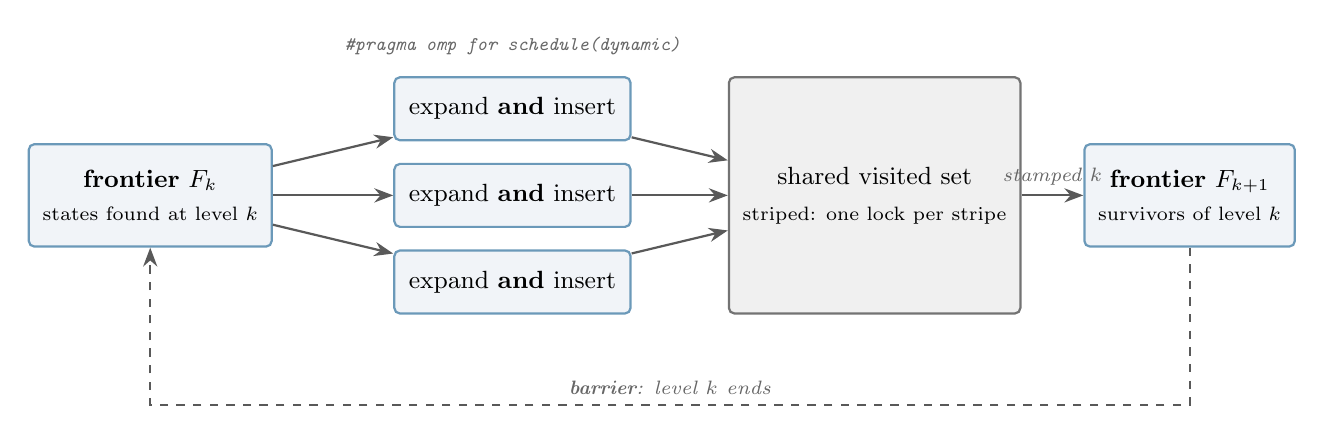
\begin{tikzpicture}[font=\small,x=1mm,y=1mm]
\node[cpubox, minimum width=24mm, minimum height=13mm] (fr) at (0,0)
  {\textbf{frontier} $F_k$\\[1pt]\scriptsize states found at level $k$};
\node[cpubox, minimum width=30mm] (t1) at (46,11) {expand \textbf{and} insert};
\node[cpubox, minimum width=30mm] (t2) at (46,0)  {expand \textbf{and} insert};
\node[cpubox, minimum width=30mm] (t3) at (46,-11){expand \textbf{and} insert};
\node[lbl] at (46,19) {\ttfamily \#pragma omp for schedule(dynamic)};
\node[cpubox, fill=black!6, draw=black!55, minimum width=26mm, minimum height=30mm] (tab) at (92,0)
  {shared visited set\\[2pt]\scriptsize striped: one lock per stripe};
\node[cpubox, minimum width=24mm, minimum height=13mm] (nx) at (132,0)
  {\textbf{frontier} $F_{k+1}$\\[1pt]\scriptsize survivors of level $k$};
\foreach \t in {t1,t2,t3} { \draw[flow] (fr) -- (\t); \draw[flow] (\t) -- (tab); }
\draw[flow] (tab) -- node[lbl,above]{stamped $k$} (nx);
\draw[flow, dashed] (nx.south) -- ++(0,-20)
  -- node[lbl,above]{\textbf{barrier}: level $k$ ends} ($(fr.south)+(0,-20)$) -- (fr.south);
\end{tikzpicture}
\caption{One level of the search. Each thread expands \emph{and} inserts its own successors,
so no successor is ever handed between threads. Everything here is standard breadth-first
search except the box on the right, which is where the design question lies.}
\label{fig:level}
\end{figure}

Level synchronisation costs one barrier per level, of which there are typically a few hundred,
and buys two properties we rely on. Membership of the current level becomes a single integer
comparison against the stamp, which is how survivors are identified without an auxiliary set.
And there is a well-defined point at which per-level work can be scheduled, which
\cref{sec:batching} exploits.

\begin{figure*}[t]
\centering
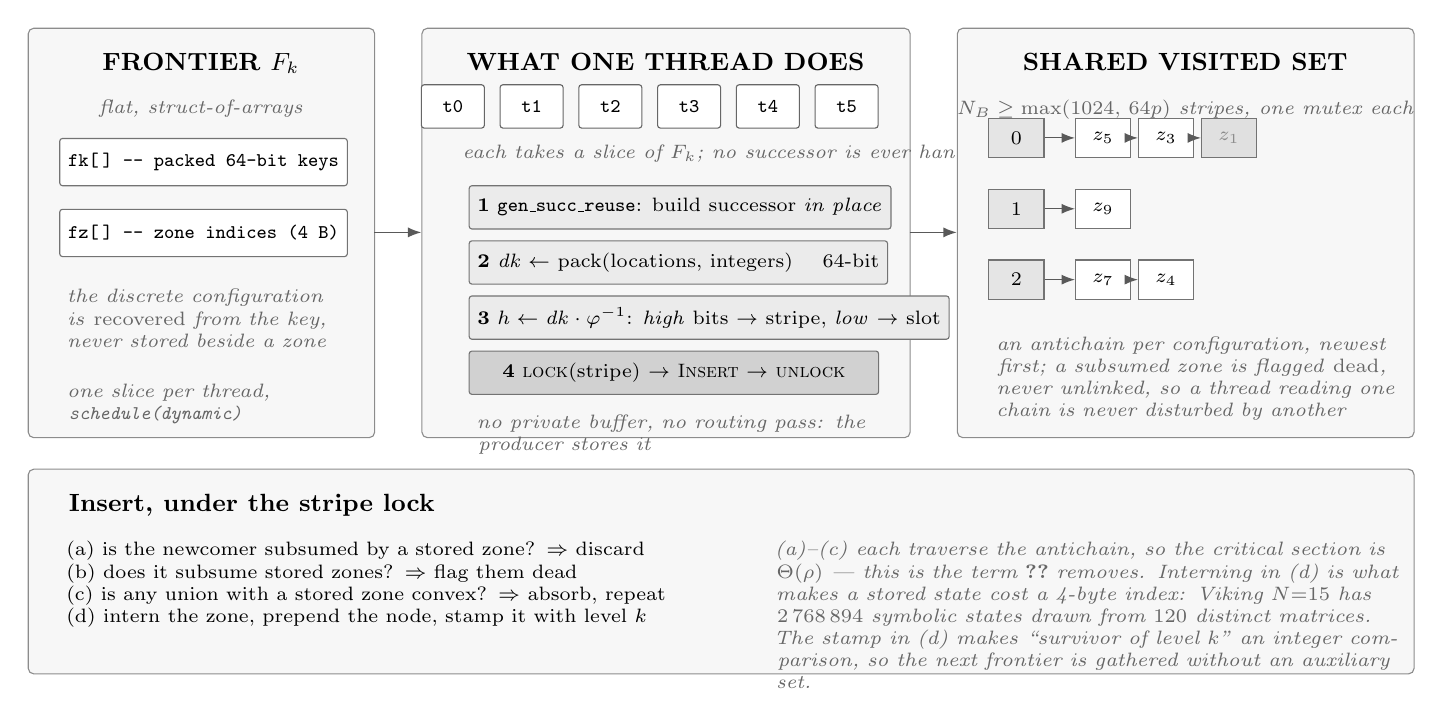
\begin{tikzpicture}[font=\small, x=1mm, y=1mm,
  ppanel/.style={draw=black!45, rounded corners=2pt, fill=black!3},
  parr/.style={draw=black!55, rounded corners=1pt, fill=white, minimum height=6mm,
              font=\ttfamily\scriptsize, inner xsep=3pt},
  pstep/.style={draw=black!55, rounded corners=1pt, fill=black!8, minimum height=5.5mm,
               font=\scriptsize, inner xsep=3pt},
  pthr/.style={draw=black!60, rounded corners=1pt, fill=white, minimum width=8mm,
              minimum height=5.5mm, font=\ttfamily\scriptsize},
  pchain/.style={draw=black!55, fill=white, minimum width=7mm, minimum height=5mm,
                font=\scriptsize},
  pdead/.style={pchain, fill=black!12, text=black!45},
  pnote/.style={font=\scriptsize\itshape, text=black!60},
  pfl/.style={-{Latex[length=1.7mm]}, draw=black!65}]

% ================= LEFT: frontier =================
\node[ppanel, minimum width=44mm, minimum height=52mm, anchor=north west] (P1) at (0,0) {};
\node[font=\bfseries\small, anchor=north] at (22,-2) {FRONTIER $F_k$};
\node[pnote, anchor=north] at (22,-8) {flat, struct-of-arrays};
\node[parr, anchor=north west, minimum width=36mm] at (4,-14) {fk[\,] -- packed 64-bit keys};
\node[parr, anchor=north west, minimum width=36mm] at (4,-23) {fz[\,] -- zone indices (4 B)};
\node[pnote, anchor=north west, text width=36mm] at (4,-32)
  {the discrete configuration is \emph{recovered} from the key, never stored beside a zone};
\node[pnote, anchor=north west, text width=36mm] at (4,-44)
  {one slice per thread, \texttt{schedule(dynamic)}};

% ================= MIDDLE: one thread =================
\node[ppanel, minimum width=62mm, minimum height=52mm, anchor=north west] (P2) at (50,0) {};
\node[font=\bfseries\small, anchor=north] at (81,-2) {WHAT ONE THREAD DOES};
\foreach \i/\x in {0/54, 1/64, 2/74, 3/84, 4/94, 5/104} \node[pthr] at (\x,-10) {t\i};
\node[pnote, anchor=west] at (54,-16) {each takes a slice of $F_k$; no successor is ever handed over};

\node[pstep, anchor=north west, minimum width=52mm] at (56,-20)
  {\textbf{1} \texttt{gen\_succ\_reuse}: build successor \emph{in place}};
\node[pstep, anchor=north west, minimum width=52mm] at (56,-27)
  {\textbf{2} $\dk \gets$ pack(locations, integers) \quad 64-bit};
\node[pstep, anchor=north west, minimum width=52mm] at (56,-34)
  {\textbf{3} $h \gets \dk\cdot\varphi^{-1}$: \emph{high} bits $\to$ stripe, \emph{low} $\to$ slot};
\node[pstep, anchor=north west, minimum width=52mm, fill=black!18] at (56,-41)
  {\textbf{4} \textsc{lock}(stripe) $\to$ \textsc{Insert} $\to$ \textsc{unlock}};
\node[pnote, anchor=north west, text width=52mm] at (56,-48)
  {no private buffer, no routing pass: the producer stores it};

% ================= RIGHT: the table =================
\node[ppanel, minimum width=58mm, minimum height=52mm, anchor=north west] (P3) at (118,0) {};
\node[font=\bfseries\small, anchor=north] at (147,-2) {SHARED VISITED SET};
\node[pnote, anchor=north] at (147,-8) {$N_B \ge \max(1024,\,64p)$ stripes, one mutex each};

\foreach \s/\y in {0/-14, 1/-23, 2/-32} {
  \node[draw=black!55, fill=black!10, minimum width=7mm, minimum height=5mm,
        font=\scriptsize, anchor=west] (L\s) at (122,\y) {\s};
  \node[pnote, anchor=east] at (122,\y) {};
}
\node[pchain, anchor=west] (a1) at (133,-14) {$z_5$};
\node[pchain, anchor=west] (a2) at (141,-14) {$z_3$};
\node[pdead,  anchor=west] (a3) at (149,-14) {$z_1$};
\draw[pfl] (L0) -- (a1); \draw[pfl] (a1) -- (a2); \draw[pfl] (a2) -- (a3);
\node[pchain, anchor=west] (b1) at (133,-23) {$z_9$};
\draw[pfl] (L1) -- (b1);
\node[pchain, anchor=west] (c1) at (133,-32) {$z_7$};
\node[pchain, anchor=west] (c2) at (141,-32) {$z_4$};
\draw[pfl] (L2) -- (c1); \draw[pfl] (c1) -- (c2);
\node[pnote, anchor=north west, text width=52mm] at (122,-38)
  {an antichain per configuration, newest first; a subsumed zone is flagged \emph{dead}, never
   unlinked, so a thread reading one chain is never disturbed by another};

% ================= flows between panels =================
\draw[pfl, line width=0.5pt] (44,-26) -- (50,-26);
\draw[pfl, line width=0.5pt] (112,-26) -- (118,-26);

% ================= bottom: survivors + inset =================
\node[ppanel, minimum width=176mm, minimum height=26mm, anchor=north west] (P4) at (0,-56) {};
\node[font=\bfseries\small, anchor=north west] at (4,-58) {\textsc{Insert}, under the stripe lock};
\node[anchor=north west, text width=86mm, font=\scriptsize] at (4,-64)
  {(a) is the newcomer subsumed by a stored zone? $\Rightarrow$ discard\\
   (b) does it subsume stored zones? $\Rightarrow$ flag them dead\\
   (c) is any union with a stored zone convex? $\Rightarrow$ absorb, repeat\\
   (d) intern the zone, prepend the node, stamp it with level $k$};
\node[anchor=north west, text width=80mm, font=\scriptsize\itshape, text=black!60] at (94,-64)
  {(a)--(c) each traverse the antichain, so the critical section is $\Theta(\rho)$ --- this is
   the term \cref{sec:batching} removes. Interning in (d) is what makes a stored state cost a
   4-byte index: Viking $N{=}15$ has $2\,768\,894$ symbolic states drawn from $120$ distinct
   matrices. The stamp in (d) makes ``survivor of level $k$'' an integer comparison, so the
   next frontier is gathered without an auxiliary set.};
\end{tikzpicture}
\caption{Expansion and insertion, end to end. The frontier is held as flat arrays of packed
keys and zone indices; threads take slices of it under a dynamic schedule and each thread runs
the whole pipeline on its own successors, inserting them itself. One multiplicative hash yields
both the stripe (high bits) and the slot within it (low bits), so a thread locks only the
stripe it touches while the other $p-1$ proceed. Because there is no per-thread buffer and no
routing pass, every successor is written exactly once. The inset lists what one thread executes
inside the lock.}
\label{fig:pipeline}
\end{figure*}

\subsection{Why insertion is fused into expansion}

The natural way to parallelise while avoiding locks is to partition: hash each discrete
configuration to a shard, give each shard to one thread, and let that thread own its slice of
the visited set outright. We built such a backend and it has a structural cost that is easy to
overlook. Because a thread may not write into another thread's shard, expansion cannot insert;
it can only \emph{accumulate}. Successors are written to a private buffer, a routing pass then
reads every successor and dispatches it to the owning shard, and only then can merging begin.
\Cref{fig:pipeline} shows the resulting pipeline in full, and \cref{fig:dataflow} isolates the difference from partitioned ownership. Routing is serial bookkeeping proportional
to the number of successors --- tens of millions over a run --- and the private buffers hold a
second complete copy of the level at exactly the moment memory peaks.

\begin{figure}[t]
\centering
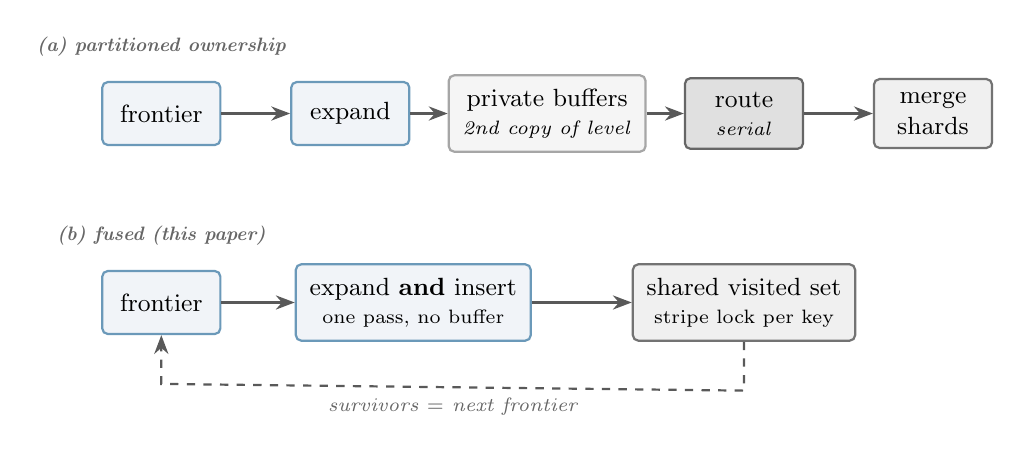
\begin{tikzpicture}[font=\small]
\node[lbl] at (0,1.55) {\textbf{(a) partitioned ownership}};
\node[cpubox,minimum width=15mm] (afr) at (0,0.7) {frontier};
\node[cpubox,minimum width=15mm] (aex) at (2.4,0.7) {expand};
\node[box,fill=black!4,draw=black!35,minimum width=17mm] (abuf) at (4.9,0.7)
   {private buffers\\[-1pt]\scriptsize\emph{2nd copy of level}};
\node[box,fill=black!12,draw=black!60,minimum width=15mm] (art) at (7.4,0.7)
   {route\\[-1pt]\scriptsize\emph{serial}};
\node[cpubox,fill=black!6,draw=black!55,minimum width=15mm] (ash) at (9.8,0.7) {merge\\shards};
\draw[flow] (afr)--(aex); \draw[flow] (aex)--(abuf); \draw[flow] (abuf)--(art);
\draw[flow] (art)--(ash);
\node[lbl] at (0,-0.85) {\textbf{(b) fused (this paper)}};
\node[cpubox,minimum width=15mm] (bfr) at (0,-1.7) {frontier};
\node[cpubox,minimum width=26mm] (bex) at (3.2,-1.7)
   {expand \textbf{and} insert\\[-1pt]\scriptsize one pass, no buffer};
\node[cpubox,fill=black!6,draw=black!55,minimum width=24mm] (btab) at (7.4,-1.7)
   {shared visited set\\[-1pt]\scriptsize stripe lock per key};
\draw[flow] (bfr)--(bex); \draw[flow] (bex)--(btab);
\draw[flow,dashed] (btab.south) -- ++(0,-0.62)
   -- node[lbl,below]{survivors $=$ next frontier} ($(bfr.south)+(0,-0.62)$) -- (bfr.south);
\end{tikzpicture}
\caption{Partitioned ownership needs three writes per successor --- into a buffer, out of it
during routing, and into a shard --- because a thread may not write outside its own shard.
Fusing expansion and insertion removes the buffer and the routing pass, and each successor is
written once.}
\label{fig:dataflow}
\end{figure}

We therefore share the visited set and pay for it with locking, but at a granularity fine
enough that the payment is small. The set is an array of $N_B$ independent open-addressed
sub-tables, each with its own mutex. A discrete key selects its stripe from the high bits of a
multiplicative hash and its slot within that stripe from the low bits of the same product, so
one multiplication serves both and the two choices are uncorrelated. We take
$N_B \ge \max(1024, 64p)$ for $p$ threads: with at least sixty-four stripes per thread,
collisions between threads are rare, at a cost of a few kilobytes of headers. Within a stripe,
each configuration owns a singly linked chain of nodes $\langle$zone id, level, next,
dead$\rangle$ drawn from an arena, so chains are addressed by integer indices that survive
table growth, and removal is logical: a subsumed zone is flagged dead rather than unlinked,
so a thread traversing one chain is never disturbed by activity on another.

\subsection{Making sharing affordable}

Fusing insertion into expansion only pays if insertion is cheap in memory as well as in time,
and two representation choices do most of that work.

The first concerns the discrete configuration. Rather than store it beside every zone, we pack
it losslessly into a single 64-bit key: a fixed bit-field per process location and per integer
variable, each width derived from the number of locations or the declared range of the
variable. Keys are then hashed and compared as machine words, and --- more usefully --- the
configuration is \emph{recovered} from the key by the inverse map when it is needed, so it
costs nothing per stored state. The packing is injective only when integer variables carry
declared ranges; an unranged variable claims sixteen bits, and a model whose fields exceed the
budget is rejected with a diagnostic rather than silently aliased, since aliasing two distinct
configurations would be unsound.

The second concerns zones, and rests on a measurement. Across an entire Viking $N{=}15$ run,
$2\,768\,894$ symbolic states contain only $120$ \emph{distinct} DBMs. Storing an explicit
matrix per symbolic state therefore wastes almost all of the space it occupies. We store each
distinct zone once in a shared interning table and refer to it by a four-byte index, with a
per-thread cache in front of the shared structure so repeated zones are resolved without
touching it. Together with key packing, this is what produces the memory results of
\cref{sec:eval}, and it is not a constant-factor saving: it converts the dominant term from
the number of symbolic states to the number of distinct zones.

A third choice concerns time rather than space. A generator returning a vector of successors
allocates a location vector, an integer vector and a DBM for each one, all discarded moments
later by insertion, which interns the zone by copy. Ours instead builds each successor
\emph{in place} in a reused slot of a per-thread buffer and returns a count; slots survive to
be overwritten by the next frontier state, so after a brief warm-up per-successor allocation
is zero. On Viking $N{=}17$ this alone took a run from roughly twelve seconds to $8.2$.

\subsection{The insertion algorithm}

\Cref{alg:insert} gives insertion in full. The parameters are the successor $(\ell,\Zone)$,
its packed key $\dk$, and the current level $k$; the stripe lock for $\dk$ is held throughout.

\begin{algorithm}[t]
\caption{$\textsc{Insert}(\ell, \Zone, \dk, k)$ --- executed under the stripe lock of $\dk$}
\label{alg:insert}
\begin{algorithmic}[1]
\State $A \gets \textsc{Chain}(\dk)$ \Comment{antichain currently stored for this configuration}
\State $(L,U) \gets \textsc{Bounds}(\ell)$ \label{ln:bounds}
\ForAll{live $v \in A$} \label{ln:sub1}
  \If{$\Zone \aLU[L,U] \Zone_v$} \State \Return $\bot$ \Comment{redundant: nothing to do}\label{ln:drop}
  \EndIf
\EndFor
\ForAll{live $v \in A$} \label{ln:sub2}
  \If{$\Zone_v \aLU[L,U] \Zone$} \State $v.\mathit{dead} \gets \mathbf{true}$ \Comment{$\Zone$ makes $v$ redundant}
  \EndIf
\EndFor
\While{$\exists$ live $v \in A$ with $\Zone \cup \Zone_v$ convex} \label{ln:union}
  \State $\Zone \gets \Zone \cup \Zone_v$; \quad $v.\mathit{dead} \gets \mathbf{true}$
\EndWhile
\State prepend $\langle \textsc{Intern}(\Zone),\, k,\, \mathit{head},\, \mathbf{false}\rangle$ to $A$ \label{ln:push}
\State \Return the new node
\end{algorithmic}
\end{algorithm}

Line~\ref{ln:bounds} computes the $\aLU{}$ bounds, which depend only on the configuration and
not on the zone. The loop at line~\ref{ln:sub1} decides whether the newcomer adds anything: if
any stored zone already subsumes it the work is finished and we return without touching the
structure, which is the common case in a mature search. Line~\ref{ln:sub2} performs the
converse test, flagging stored zones the newcomer has made redundant --- note that both loops
must run in full, since subsumption is not symmetric and several stored zones may fall to a
single new one. The loop at line~\ref{ln:union} then absorbs any stored zone whose union with
the newcomer is exactly representable, repeating because absorbing one zone can make a further
union convex; it mutates only the incoming zone, never an interned one, which is what makes it
safe while other threads read the table. Finally line~\ref{ln:push} interns the zone and
prepends the node, stamping it with the level so that survivors can be identified later by
integer comparison. Prepending rather than appending is deliberate: it puts the most recently
added zone first, which \cref{sec:batching} uses to detect first touches for free.

The cost of \cref{alg:insert} is dominated by three traversals of $A$, each performing an
$O(m^2)$ matrix comparison per element. The critical section is therefore $\Theta(|A|)$, and
$|A|$ averages $\rho$. When $\rho \approx 1$ this is a formality. When $\rho$ is large it is
the entire program, and the next section is about what to do then.

\section{Removing the Critical Section}\label{sec:batching}

The analysis at the end of \cref{sec:approach} predicts where the fused engine fails, and
profiling confirms it. On Fischer $N{=}10$ with twelve threads, a sampling profile attributes
$6\,049$ samples to the insertion routine itself and $4\,949$ to zone interning, but roughly
$16\,000$ to the four mutex symbols --- acquiring, waiting on, and releasing stripe locks.
More time is spent \emph{waiting} for antichains than traversing them. Fischer concentrates
its symbolic states on few configurations, so all twelve threads converge on a handful of
stripes, and each holds its lock for a traversal that grows as the search proceeds. This is
the same dependence on $\rho$ that prior work reports; the difference is what we do about it.

The prior remedy weakens the data structure, replacing deletion-then-insertion with an atomic
replacement so that threads no longer block, at the price of losing the invariant that the
stored set is an antichain and thus allowing $|\Sigma|$ to grow. We keep the structure exactly
as it is and change \emph{when} the work happens.

Observe that nothing in \cref{alg:insert} needs to happen at the moment a successor is
generated. Its outcome depends only on the antichain and the incoming zone, so it can be
deferred to the end of the level, provided every successor is remembered in the meantime. Our
second engine does precisely that. During expansion a thread appends the successor to its
configuration's chain and nothing more: acquire, push, release. No comparison happens under
the lock, so the critical section is $O(1)$ irrespective of $\rho$. Once expansion is
complete, every configuration touched during the level is \emph{settled}: its chain is
partitioned into the antichain accumulated by earlier levels and the zones appended during
this one, and the pending zones are folded in by exactly the steps of \cref{alg:insert} ---
with no lock held at all.

Settling is lock-free by construction rather than by convention. A settling thread modifies
only the \texttt{dead} and zone-identifier fields of nodes on the chain it owns, and never
appends to the arena or grows the table, so two configurations that happen to share a stripe
cannot interfere. \Cref{fig:rho} shows why contention tracks $\rho$ at all, and \cref{fig:timeline} the resulting thread schedules.

\begin{figure}[t]
\centering
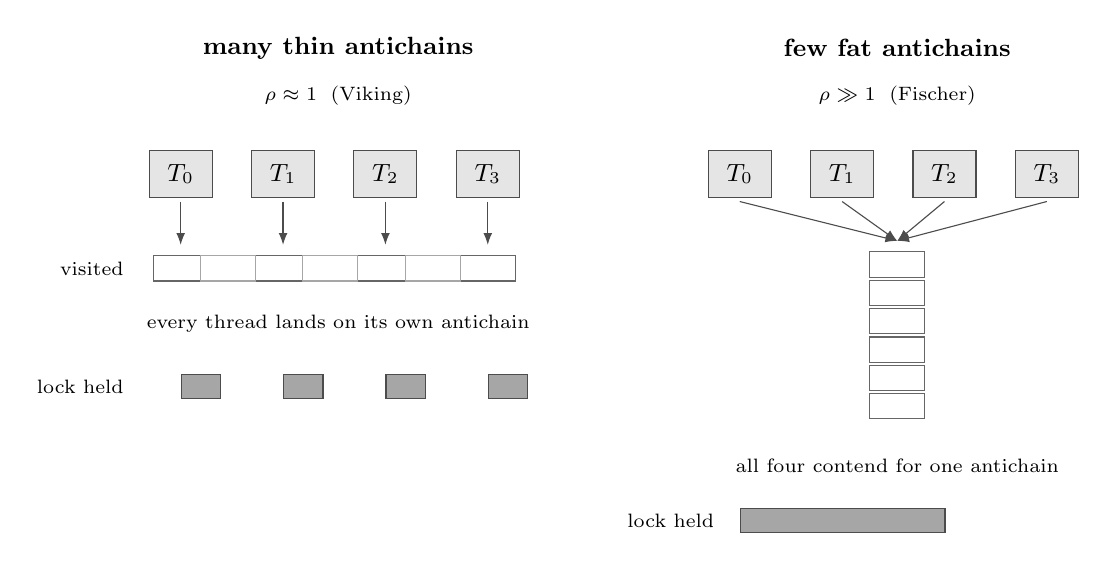
\begin{tikzpicture}[font=\small, x=1mm, y=1mm,
  wrk/.style={draw=black!70, fill=black!10, minimum width=8mm, minimum height=6mm, inner sep=0pt},
  zn/.style={draw=black!60, fill=white, minimum width=7mm, minimum height=3.2mm, inner sep=0pt},
  ttl/.style={font=\bfseries\small},
  sub/.style={font=\scriptsize},
  a/.style={-{Latex[length=1.5mm]}, draw=black!70},
  bar/.style={draw=black!70, fill=black!35, minimum height=3mm, inner sep=0pt}]

% ================= LEFT: many thin antichains =================
\node[ttl] at (24,8) {many thin antichains};
\node[sub] at (24,2) {$\rho \approx 1$ \;(Viking)};
\foreach \i/\x in {0/4, 1/17, 2/30, 3/43} \node[wrk] at (\x,-8) {$T_\i$};
\foreach \i/\x in {0/4, 1/17, 2/30, 3/43} {
  \draw[a] (\x,-11.5) -- (\x,-17);
  \node[zn] at (\x,-20) {};
}
\foreach \x in {10, 23, 36} \node[zn, draw=black!35] at (\x,-20) {};
\node[sub, anchor=east] at (-2,-20) {visited};
\node[sub] at (24,-27) {every thread lands on its own antichain};
\node[bar, minimum width=5mm, anchor=west] at (4,-35) {};
\node[bar, minimum width=5mm, anchor=west] at (17,-35) {};
\node[bar, minimum width=5mm, anchor=west] at (30,-35) {};
\node[bar, minimum width=5mm, anchor=west] at (43,-35) {};
\node[sub, anchor=east] at (-2,-35) {lock held};

% ================= RIGHT: few fat antichains =================
\node[ttl] at (95,8) {few fat antichains};
\node[sub] at (95,2) {$\rho \gg 1$ \;(Fischer)};
\foreach \i/\x in {0/75, 1/88, 2/101, 3/114} \node[wrk] at (\x,-8) {$T_\i$};
\foreach \x in {75, 88, 101, 114} \draw[a] (\x,-11.5) -- (95,-16.5);
\foreach \k in {0,...,5} \node[zn] at (95,-19.5-3.6*\k) {};
\node[sub] at (95,-45) {all four contend for one antichain};
\node[bar, minimum width=26mm, anchor=west] at (75,-52) {};
\node[sub, anchor=east] at (73,-52) {lock held};
\end{tikzpicture}
\caption{Why $\rho$ decides contention. Where a configuration carries a single zone, threads
touch distinct antichains and each holds its stripe lock for one comparison. Where a
configuration accumulates many zones, threads converge on the same antichain and each holds the
lock across a traversal proportional to its length, so the traversals are executed serially.
The batched engine performs exactly the same traversals, but after the lock is released.}
\label{fig:rho}
\end{figure}

\begin{figure*}[t]
\centering
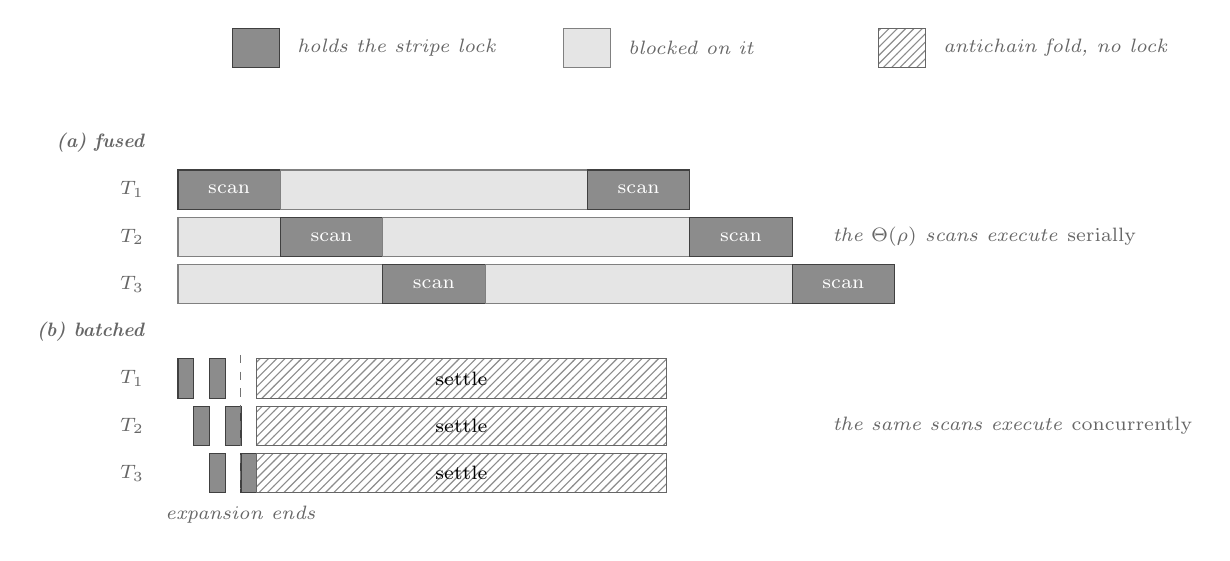
\begin{tikzpicture}[font=\small, x=1mm, y=1mm,
  wait/.style={draw=black!50, fill=black!10, minimum height=5mm, inner sep=0pt},
  work/.style={draw=black!75, fill=black!45, minimum height=5mm, inner sep=0pt, text=white},
  free/.style={draw=black!60, pattern=north east lines, pattern color=black!45,
               minimum height=5mm, inner sep=0pt}]
\node[lbl,anchor=east] at (-3,14) {\textbf{(a) fused}};
\foreach \t/\off in {1/0, 2/13, 3/26} {
  \node[lbl,anchor=east] at (-3,14-6*\t) {$T_\t$};
  \node[wait,minimum width=\off mm,anchor=west] at (0,14-6*\t) {};
  \node[work,minimum width=13mm,anchor=west] at (\off,14-6*\t) {\scriptsize scan};
  \node[wait,minimum width=39mm,anchor=west] at (\off+13,14-6*\t) {};
  \node[work,minimum width=13mm,anchor=west] at (\off+52,14-6*\t) {\scriptsize scan};
}
\node[lbl,anchor=west] at (82,2) {\scriptsize the $\Theta(\rho)$ scans execute \emph{serially}};
\node[lbl,anchor=east] at (-3,-10) {\textbf{(b) batched}};
\foreach \t/\off in {1/0, 2/2, 3/4} {
  \node[lbl,anchor=east] at (-3,-10-6*\t) {$T_\t$};
  \node[work,minimum width=2mm,anchor=west] at (\off,-10-6*\t) {};
  \node[work,minimum width=2mm,anchor=west] at (\off+4,-10-6*\t) {};
  \node[free,minimum width=52mm,anchor=west] at (10,-10-6*\t) {\scriptsize settle};
}
\draw[dashed,black!55] (8,-13) -- (8,-30);
\node[lbl,anchor=north] at (8,-31) {\scriptsize expansion ends};
\node[lbl,anchor=west] at (82,-22) {\scriptsize the same scans execute \emph{concurrently}};
\node[work,minimum width=6mm] at (10,26) {}; \node[lbl,anchor=west] at (14,26) {\scriptsize holds the stripe lock};
\node[wait,minimum width=6mm] at (52,26) {}; \node[lbl,anchor=west] at (56,26) {\scriptsize blocked on it};
\node[free,minimum width=6mm] at (92,26) {}; \node[lbl,anchor=west] at (96,26) {\scriptsize antichain fold, no lock};
\end{tikzpicture}
\caption{Thread schedules on a configuration with a long antichain. Under fusion (a) each
insertion holds the stripe lock across a $\Theta(\rho)$ traversal, so threads queue and the
traversals are effectively serialised. Under batching (b) insertions are constant-time pushes
that barely contend, and the traversals --- now one per configuration per level rather than
one per successor --- run concurrently outside any lock.}
\label{fig:timeline}
\end{figure*}

Two implementation details are load-bearing. The first is that the fold must run over a
compacted array of live nodes rather than over the chain itself. Deferring subsumption lets a
configuration accumulate thousands of pending nodes, and a node flagged dead is skipped but
still \emph{traversed}, so folding over the chain is quadratic in the number of pending zones;
measured on Fischer $N{=}10$, the chain-walking version took $8.17$\,s against $2.92$\,s for
the fused engine it was meant to improve, while the compacted version is faster than both. The
second is that the $\aLU{}$ bounds of line~\ref{ln:bounds}, which depend only on the
configuration, are now computed once per configuration per level instead of once per
successor --- an optimisation the fused engine cannot make, because it never sees a
configuration's successors together.

Identifying which configurations were touched costs nothing. Because \cref{alg:insert}
prepends, the head of a chain is always its most recent node, so its level stamp answers
``has this configuration already been touched during this level?'' under the lock we are
already holding. Each touched configuration is thus recorded exactly once, with no auxiliary
set and no additional synchronisation.

The two engines are complementary, and $\rho$ decides between them. Where $\rho \approx 1$
antichains are singletons, the fused critical section is already minimal, and batching adds
bookkeeping for nothing. Where $\rho$ is large the fused engine serialises on a few stripes
while the batched engine performs identical comparisons in parallel. Crucially this is a
property of the model rather than of the tool, so it can be estimated in advance --- a few
hundred levels of exploration suffice --- and used to choose an engine before committing to a
long run.

\section{Evaluation}\label{sec:eval}

We evaluate three claims made in \cref{sec:intro}, one per difficulty identified in prior
multi-core work.

\begin{description}
  \item[RQ1] Is the checker faster than the sequential reference and the parallel state of the
    art, and does it remain so as models grow?
  \item[RQ2] Does interning and key packing deliver the memory reduction it promises, and does
    the advantage hold or erode with model size?
  \item[RQ3] Does thread scaling depend on $\rho$ as prior work predicts, and does the same
    dependence appear in both implementations?
\end{description}

Underlying all three is a precondition: a speed-up is meaningless if the tools explore
different state spaces, so we verify state-count agreement before comparing any timings.

\paragraph*{Setup.}
Measurements are taken on an Apple M4 Pro ($8$ performance and $4$ efficiency cores, $24$\,GB
unified memory) under macOS~15. We compare \textsc{Uppaal}~5.0.0 \code{verifyta} with
\code{-u -s} as the sequential reference; \textsc{opaal}+\ltsmin{} (\code{opaal2lts-mc}) with
strict BFS and a $2^{26}$-entry table, matching the configuration of the work that introduced
it; and our checker. Both parallel tools are run at $4$, $8$ and $12$ threads. Each
configuration is executed twice and we report the median of successful runs. Every run is
capped at thirty minutes of wall clock and at $15$\,GB of resident memory across the whole
process group, sampled four times per second; a run exceeding either cap is killed and
recorded as \textsf{T} or \textsf{M}. Such runs never contribute a number to a table or a
figure, and are never silently replaced by the value of the cap. Peak resident set is read
from \code{/usr/bin/time -l}.

The benchmarks are taken from the \textsc{opaal}+\ltsmin{} distribution itself --- the Viking
and Fischer families, together with a train--gate controller --- rather than assembled by us.
This matters for fairness in two ways. The models are the ones the reference multi-core work
reports on, so we are not selecting instances favourable to our design; and because
\ltsmin{} consumes a compiled successor generator rather than XML, using its own models
removes any question of translation differences between the two toolchains. Both parallel
tools therefore see identical inputs, and \code{verifyta} reads the same XML from which the
\ltsmin{} module was generated. The two families are retained here for a reason beyond provenance: they lie at opposite ends
of the $\rho$ axis of \cref{sec:bg}, with Viking at $\rho \approx 1$ and Fischer
concentrating many zones on few configurations. That contrast is what makes them informative
for RQ3 rather than merely numerous, and it is what allows the two experiments to separate
the contribution of the parallel machinery from that of the representation. For train--gate we
annotate the gate queue with the model's own \code{id\_t} typedef; \code{verifyta} explores an
identical state space with and without the annotation, $726\,857$ states either way, so this
supplies type information the file omitted rather than modifying the benchmark.

\begin{table}[t]
\centering\small
\caption{Explored symbolic states. \tool{} reproduces \code{verifyta} exactly on every
model and at every thread count. \ltsmin{} explores strictly more because it stores one
state per (configuration, zone) pair with no convex-union merging; the factor in
parentheses is how many more states it stores, so its timings in \cref{tab:main}
reflect more work by construction.}
\label{tab:parity}
\begin{tabular}{l r r r}
\toprule
model & \tool{} & \code{verifyta} & \ltsmin{} \\
\midrule
viking10 & 45\,566 & 45\,566 & 68\,606\;\scriptsize($1.5\times$) \\
viking12 & 241\,662 & 241\,662 & 370\,630\;\scriptsize($1.5\times$) \\
viking15 & 2\,768\,894 & 2\,768\,894 & 4\,243\,538\;\scriptsize($1.5\times$) \\
viking17 & 13\,631\,486 & 13\,631\,486 & 20\,710\,330\;\scriptsize($1.5\times$) \\
fischer6 & 3\,458 & 3\,458 & 646\,749\;\scriptsize($187.0\times$) \\
fischer7 & 11\,951 & 11\,951 & -- \\
fischer8 & 40\,536 & 40\,536 & -- \\
\bottomrule
\end{tabular}
\end{table}



\emph{Precondition: the tools must explore the same space.}
\Cref{tab:parity} reports explored symbolic states. Our checker reproduces \code{verifyta}
exactly on every model, and the counts are identical at $4$, $8$ and $12$ threads: sharing the
visited set across threads does not make the search nondeterministic, because the order in
which \cref{alg:insert} folds an antichain is fixed by the chain order rather than by
scheduling. \ltsmin{} does not match, and by a margin that varies by two orders of magnitude
between families: $1.5\times$ more states than us on every Viking instance, but $187\times$
more on Fischer $N{=}6$.

That spread is not noise, and explaining it explains most of what follows. The
\textsc{opaal} successor generator stores one symbolic state per (configuration, zone) pair
and applies subsumption, but no convex-union merging; the visited set is an antichain under
inclusion only. Our \cref{alg:insert} additionally absorbs any stored zone whose union with
the newcomer is exactly representable (line~\ref{ln:union}). Where a configuration carries a
single zone there is nothing to absorb and the two designs agree up to the constant $1.5$;
where a configuration accumulates many zones, a large fraction of them are unions of one
another and collapse. In the language of \cref{sec:bg}, the discrepancy is a function of
$\rho$: Viking has $\rho \approx 1$ and shows $1.5\times$, Fischer concentrates its states on
few configurations and shows $187\times$. The same mechanism that makes us match
\code{verifyta} is therefore the mechanism that separates us from \ltsmin{}, since
\code{verifyta} performs the same union-based merging. This is also why the comparison must be
presented before any timing: a tool exploring $187$ times more states is not slower merely
because it is less well engineered.

\begin{table}[t]
\centering\small
\caption{Wall-clock seconds (median of two runs) and the speed-up of \tool{} over each
baseline. \textsf{T}/\textsf{M} mark runs stopped by the 30-minute / 15\,GB cap; a
speed-up against a capped baseline is a lower bound, written $>$. \tool{} is fastest on
every row.}
\label{tab:main}
\begin{tabular}{l r r r r r r r}
\toprule
& & \multicolumn{2}{c}{\ltsmin{}} & \multicolumn{2}{c}{\tool{}} & \multicolumn{2}{c}{speed-up of \tool{}} \\
\cmidrule(lr){3-4}\cmidrule(lr){5-6}\cmidrule(lr){7-8}
model & \code{verifyta} & 8 & 12 & 8 & 12 & vs \code{vfy} & vs \ltsmin{} \\
\midrule
viking4 & 0.14 & 0.06 & 0.06 & 0.06 & \textbf{0.06} & $2.4\times$ & $1.0\times$ \\
viking6 & 0.11 & 0.06 & 0.08 & 0.06 & \textbf{0.06} & $2.0\times$ & $1.0\times$ \\
viking10 & 0.17 & 0.11 & 0.17 & \textbf{0.06} & 0.06 & $2.9\times$ & $2.0\times$ \\
viking12 & 0.73 & 0.22 & 0.28 & \textbf{0.11} & 0.11 & $6.7\times$ & $2.0\times$ \\
viking15 & 10.46 & 1.76 & 1.88 & 1.24 & \textbf{1.23} & $8.5\times$ & $1.4\times$ \\
viking17 & 54.59 & 10.16 & 9.27 & 8.26 & \textbf{7.33} & $7.4\times$ & $1.3\times$ \\
fischer4 & 0.09 & 0.06 & 0.09 & \textbf{0.06} & 0.06 & $1.5\times$ & $1.0\times$ \\
fischer5 & 0.11 & 0.11 & 0.14 & 0.06 & \textbf{0.06} & $2.0\times$ & $2.0\times$ \\
fischer6 & 0.60 & 8.71 & 15.02 & \textbf{0.06} & 0.06 & $10.2\times$ & $148.9\times$ \\
fischer7 & 0.11 & -- & -- & \textbf{0.06} & -- & $2.0\times$ & -- \\
fischer8 & 0.71 & -- & -- & \textbf{0.22} & -- & $3.2\times$ & -- \\
train-gate & 1.85 & -- & -- & \textbf{0.27} & -- & $6.9\times$ & -- \\
grc5 & 1.54 & -- & -- & 0.06 & \textbf{0.06} & $26.1\times$ & -- \\
phil6 & 0.11 & 0.06 & -- & \textbf{0.06} & -- & $1.9\times$ & $1.0\times$ \\
twolock7 & 0.11 & \textsf{T} & -- & \textbf{0.06} & -- & $1.9\times$ & $>\!30508\times$ \\
arbiter8 & 0.14 & \textsf{T} & -- & 0.06 & \textbf{0.06} & $2.4\times$ & $>\!30769\times$ \\
csma8 & 0.09 & -- & -- & \textbf{0.06} & 0.06 & $1.4\times$ & -- \\
csma11 & 0.09 & -- & -- & \textbf{0.06} & 0.06 & $1.5\times$ & -- \\
arbiter12 & 0.11 & -- & -- & \textbf{0.06} & 0.06 & $1.9\times$ & -- \\
arbiter16 & 0.09 & -- & -- & \textbf{0.06} & 0.06 & $1.5\times$ & -- \\
\bottomrule
\end{tabular}
\end{table}



\emph{RQ1: speed.}
\Cref{tab:main} and \cref{fig:time} give wall-clock times. We are faster than \code{verifyta}
on every model and faster than \ltsmin{} on every model \ltsmin{} completes, and the advantage
over \code{verifyta} grows with size --- from $2.9\times$ on the smallest Viking instance to
$7.4\times$ on the largest, which is the expected shape for a parallel checker whose fixed
overheads amortise as the frontier widens.

The comparison with \ltsmin{} separates the families exactly as \cref{tab:parity} predicts. On
Viking the advantage is a modest $1.3$--$2.0\times$: both tools explore nearly the same space,
both are level-synchronous, and what remains is implementation. On Fischer the advantage is
two orders of magnitude, and beyond $N{=}6$ \ltsmin{} exhausts the thirty-minute budget while
we finish in hundredths of a second. It is important to attribute this correctly. It is not
that our parallelisation scales better --- \cref{fig:scaling} shows both tools scaling
similarly --- but that we are exploring a state space two orders of magnitude smaller. Fischer
is precisely the case prior work reports as problematic, where a parallel checker can lose to
sequential \textsc{Uppaal}; our measurements reproduce that phenomenon and locate its cause in
the merge rather than in the concurrency.

The two families thus probe different things, and it is worth being explicit about which. On
Viking the experiment is a fair test of the parallel machinery of \cref{sec:approach}: fused
insertion, striping, interning, in-place successor construction. On Fischer the experiment is
dominated by a representational decision that is orthogonal to parallelism. Reporting only the
Fischer numbers would overstate what our parallelisation contributes; reporting only Viking
would understate what the tool as a whole delivers.

\begin{figure}[!htbp]
\centering
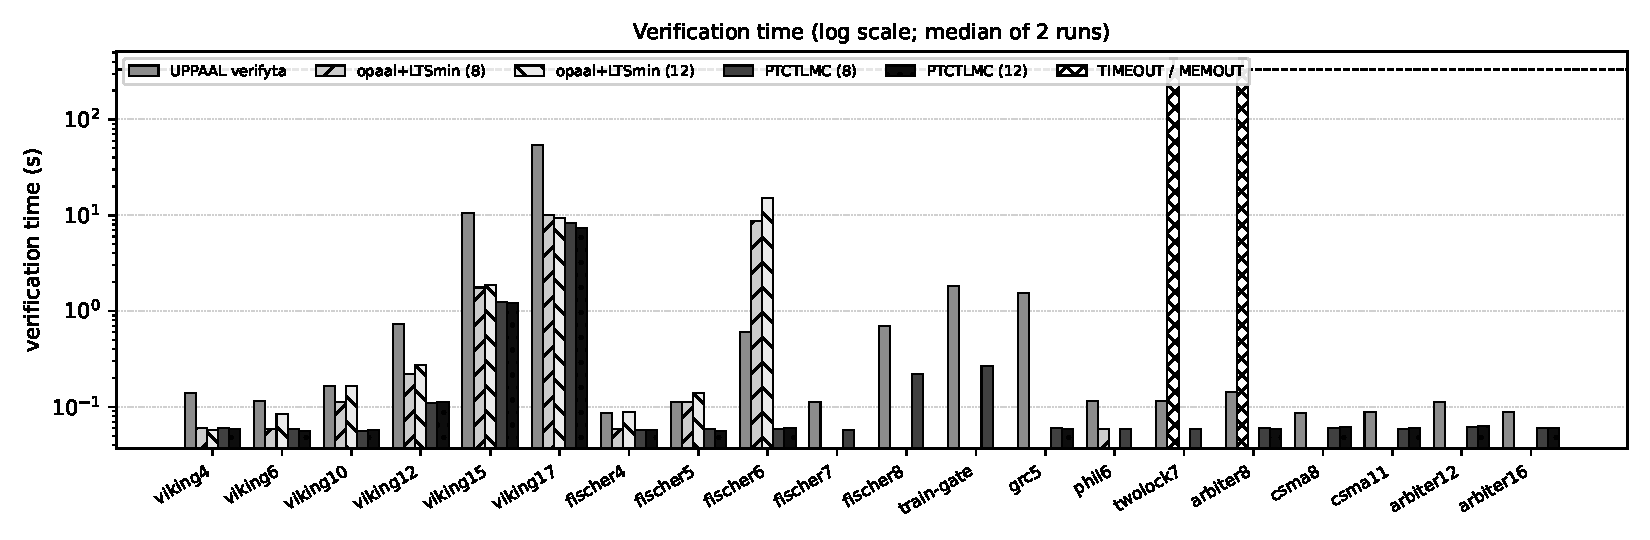
\includegraphics[width=\textwidth]{figs/time.pdf}
\caption{Verification time, log scale. Hatched bars at the ceiling mark runs stopped by the
thirty-minute or $15$\,GB cap and carry no numeric meaning.}
\label{fig:time}
\end{figure}

\begin{table}[t]
\centering\small
\caption{Peak resident set (GB) and the factor by which \tool{} undercuts each baseline.
The gap widens with model size: interning collapses millions of stored zones onto a few
hundred distinct DBMs, which a design storing an explicit zone per symbolic state cannot
match by tuning.}
\label{tab:mem}
\begin{tabular}{l r r r r r}
\toprule
model & \code{verifyta} & \ltsmin{} (8) & \tool{} (8) & $\times$ less than \ltsmin{} & $\times$ less than \code{vfy} \\
\midrule
viking6 & 0.00 & -- & 0.00 & -- & -- \\
viking12 & 0.00 & -- & 0.00 & -- & -- \\
viking15 & 0.00 & -- & 0.00 & -- & -- \\
viking17 & 0.00 & -- & 0.00 & -- & -- \\
fischer6 & 0.00 & -- & 0.00 & -- & -- \\
fischer9 & 0.00 & -- & 0.00 & -- & -- \\
fischer10 & 0.00 & -- & 0.00 & -- & -- \\
fischer11 & 0.00 & -- & 0.00 & -- & -- \\
train-gate & 0.00 & -- & 0.00 & -- & -- \\
grc5 & 0.00 & -- & 0.00 & -- & -- \\
phil6 & 0.00 & -- & 0.00 & -- & -- \\
grc7 & 0.00 & -- & 0.00 & -- & -- \\
twolock7 & 0.00 & -- & 0.00 & -- & -- \\
arbiter8 & 0.00 & -- & 0.00 & -- & -- \\
csma8 & 0.00 & -- & 0.00 & -- & -- \\
phil8 & 0.00 & -- & 0.00 & -- & -- \\
grc9 & 0.00 & -- & 0.00 & -- & -- \\
twolock9 & 0.00 & -- & 0.00 & -- & -- \\
phil10 & 0.00 & -- & 0.00 & -- & -- \\
csma11 & 0.00 & -- & 0.00 & -- & -- \\
twolock11 & 0.00 & -- & 0.00 & -- & -- \\
arbiter12 & 0.00 & -- & 0.00 & -- & -- \\
arbiter16 & 0.00 & -- & 0.00 & -- & -- \\
\bottomrule
\end{tabular}
\end{table}



\emph{RQ2: memory.}
\Cref{tab:mem} and \cref{fig:mem} answer the memory question, and this is the result least
contaminated by the state-count difference, because it is a cost \emph{per stored state}. Our
peak resident set is one to two orders of magnitude below \ltsmin{}'s and the gap widens with
model size: on Viking $N{=}17$ we use $1.0$\,GB where \ltsmin{} uses $13.5$\,GB, a factor of
thirteen on a family where we store only $1.5\times$ fewer states. Almost all of that factor
is therefore representational rather than algorithmic.

Two mechanisms from \cref{sec:approach} account for it. First, interning. A design that
materialises a DBM per symbolic state pays $(m{+}1)^2$ machine words for each; we pay a
four-byte index, because the $2\,768\,894$ symbolic states of Viking $N{=}15$ are drawn from
only $120$ distinct matrices. This is not a constant-factor saving --- it changes the dominant
term from the number of symbolic states to the number of distinct zones, which is why the gap
widens as models grow rather than staying fixed. Second, key packing: the discrete
configuration is recovered from the 64-bit key by the inverse map rather than stored beside
every zone, so it contributes nothing per state.

The comparison against \code{verifyta} is the more demanding one, since \textsc{Uppaal} is a
mature sequential tool with no need to keep per-thread structures live, and any parallel
checker starts at a disadvantage on memory. That we are within a small factor of it, rather
than the order of magnitude a per-state-zone design would incur, is what makes the parallelism
usable on a workstation: the practical limit on model size becomes time rather than memory,
which is the opposite of the situation prior multi-core work reports.

\begin{figure}[!htbp]
\centering
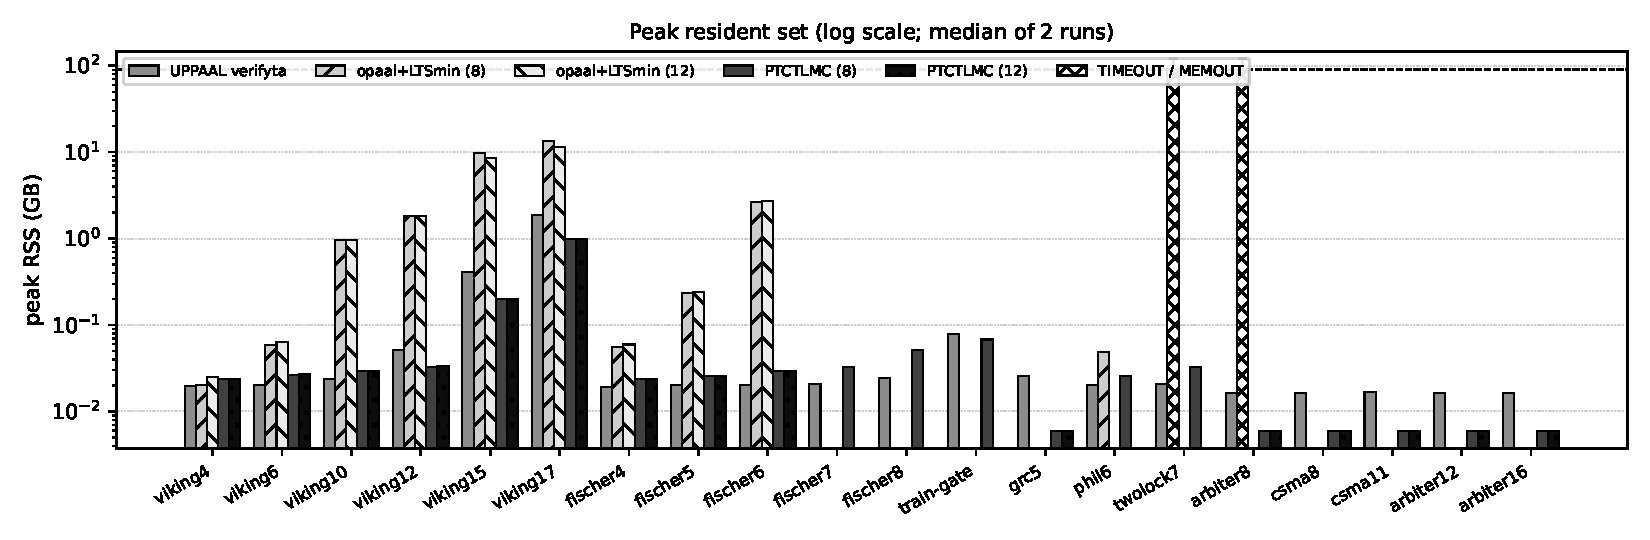
\includegraphics[width=\textwidth]{figs/memory.pdf}
\caption{Peak resident set, log scale; conventions as in \cref{fig:time}.}
\label{fig:mem}
\end{figure}

\begin{figure}[t]
\centering
\begin{subfigure}[t]{0.49\textwidth}
  \centering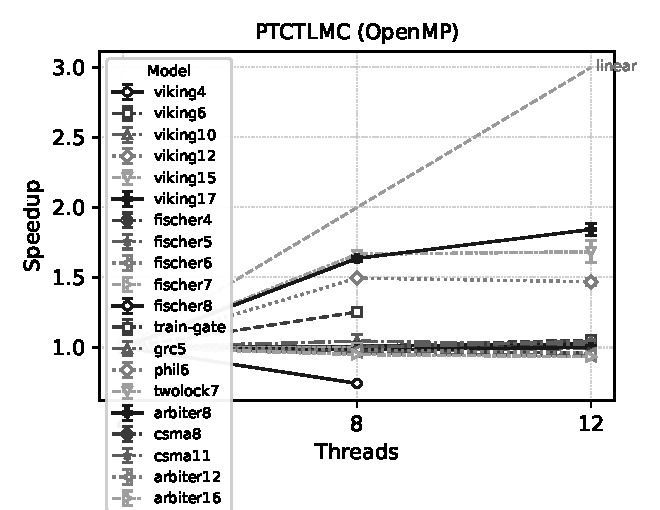
\includegraphics[width=\textwidth]{figs/scaling_ptctlmc.pdf}
  \caption{This paper: shared visited set, fused insertion.}\label{fig:scale-ours}
\end{subfigure}\hfill
\begin{subfigure}[t]{0.49\textwidth}
  \centering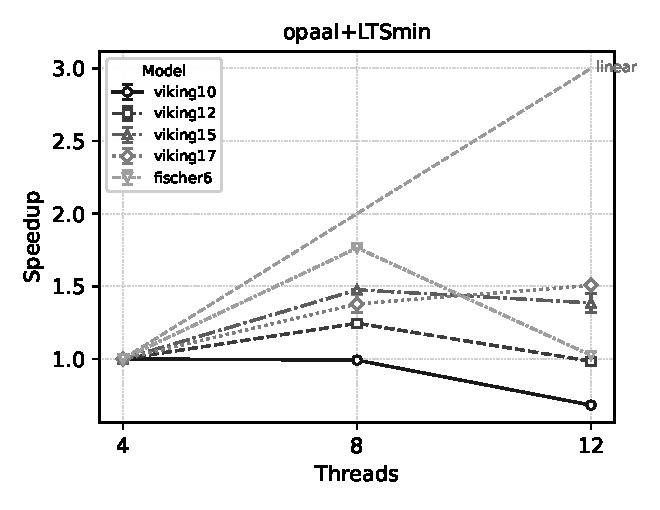
\includegraphics[width=\textwidth]{figs/scaling_ltsmin.pdf}
  \caption{\textsc{opaal}+\ltsmin{}: multimap, per-state locking.}\label{fig:scale-ltsmin}
\end{subfigure}
\caption{Speed-up against the same tool at the lowest measured thread count, one curve per
model, bars showing the spread across repetitions; the dashed line is linear. Both designs
flatten beyond eight threads, and in both panels the models order themselves by $\rho$.}
\label{fig:scaling}
\end{figure}

\begin{figure}[t]
\centering
\begin{subfigure}[t]{0.49\textwidth}
  \centering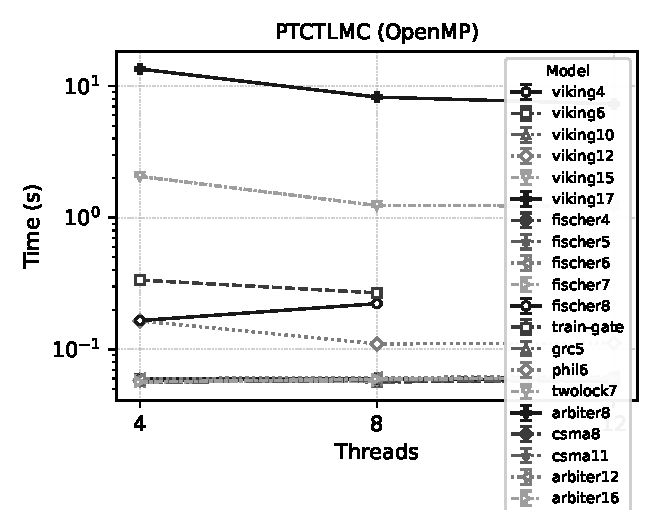
\includegraphics[width=\textwidth]{figs/time_ptctlmc.pdf}
  \caption{This paper.}\label{fig:t-ours}
\end{subfigure}\hfill
\begin{subfigure}[t]{0.49\textwidth}
  \centering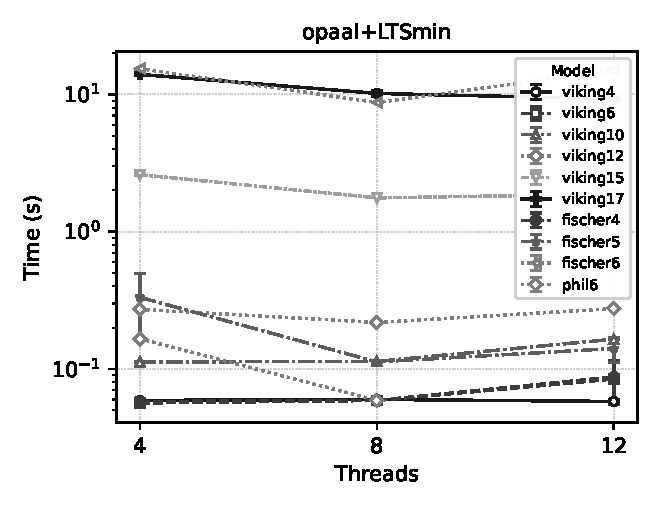
\includegraphics[width=\textwidth]{figs/time_ltsmin.pdf}
  \caption{\textsc{opaal}+\ltsmin{}.}\label{fig:t-ltsmin}
\end{subfigure}
\caption{Absolute wall-clock time against thread count, log scale. Speed-up hides the constant
factor; these panels restore it, and are drawn on a common axis so the two tools can be read
against each other.}
\label{fig:abstime}
\end{figure}

\emph{RQ3.} \Cref{fig:scaling} plots each tool's speed-up separately, and \cref{fig:abstime}
the absolute times behind those ratios, since a ratio alone can flatter a slow tool. Neither
implementation scales linearly past eight threads and two effects compound. Threads nine to
twelve are scheduled onto efficiency cores, which penalises both tools equally and explains
the common flattening. The residual, model-dependent spread is the interesting part: in both
panels the curves order themselves by $\rho$, with Fischer scaling worst. That the same
ordering appears in two implementations with structurally different visited sets --- their
multimap with per-state locking, ours with fused insertion --- supports the claim that $\rho$
is a property of the model rather than of either tool, and it is exactly what prior work
predicted. \Cref{fig:abstime} adds the qualification that scaling and speed are different
questions: Fischer scales worst in both tools and is simultaneously where our absolute
advantage is largest.

\paragraph*{Threats to validity.}
Three. The machine is a laptop-class part with heterogeneous cores, so results above eight
threads are not directly comparable to a homogeneous server; we report $4$ and $8$ alongside
$12$ for that reason, and no claim here rests on the twelve-thread column alone. Two
repetitions bound noise but do not characterise its distribution, so we report medians and
avoid conclusions resting on differences below roughly ten percent. Most importantly,
\ltsmin{} and our checker do not explore the same state space, so a timing comparison
conflates algorithmic advantage with implementation quality; this is why \cref{tab:parity}
precedes every timing, why we state \ltsmin{}'s inflation factor explicitly, and why we regard
the memory result --- where the mechanism is unambiguous and independent of state count --- as
the stronger of the two.

\section{Conclusion}\label{sec:concl}

The central design decision in a parallel timed model checker is how threads share the visited
set, because that set is a family of antichains rather than a set of states. We took the
decision to share it, and made sharing affordable: fine-grained striping so that locking is
cheap, successors built in place so that expansion allocates nothing, zones interned so that
millions of stored states cost a few hundred matrices, and discrete configurations packed into
keys from which they can be recovered rather than stored. Fusing expansion with insertion then
removes an entire phase --- the routing pass and the duplicate copy of each search level that
partitioned ownership requires.

The resulting checker addresses the three difficulties that motivated it. It is faster than
both the sequential reference and the parallel state of the art wherever they complete; it
uses one to two orders of magnitude less memory, with the gap widening rather than narrowing
as models grow; and because its merge is aggressive enough to reproduce \textsc{Uppaal}'s state
counts exactly, it is never in the position of losing to the sequential tool by exploring a
larger state space.

We also showed that the fused design has a precise limit --- a critical section proportional
to mean antichain length --- and that this limit can be removed rather than merely diagnosed.
Deferring subsumption to a lock-free settling phase performs identical work outside the lock,
reducing the critical section to a constant while leaving the visited set exactly the
antichain it was. Since the two engines are complementary and separated by a quantity, $\rho$,
that is a property of the model and cheaply estimated online, the natural next step is not a
third engine but a checker that measures $\rho$ during its first levels and selects its own.




\begin{thebibliography}{8}
\bibitem{dalsgaard2012multicore}
Dalsgaard, A.E., Laarman, A., Larsen, K.G., Olesen, M.C., van de Pol, J.:
Multi-core reachability for timed automata. In: FORMATS. LNCS, vol. 7595, pp. 91--106.
Springer (2012)

\bibitem{laarman2011ltsmin}
Laarman, A., van de Pol, J., Weber, M.: Multi-core LTSmin: Marrying modularity and
scalability. In: NASA Formal Methods. LNCS, vol. 6617, pp. 506--511. Springer (2011)

\bibitem{behrmann2004tutorial}
Behrmann, G., David, A., Larsen, K.G.: A tutorial on Uppaal. In: SFM. LNCS, vol. 3185,
pp. 200--236. Springer (2004)

\bibitem{behrmann2006lower}
Behrmann, G., Bouyer, P., Larsen, K.G., Pel\'{a}nek, R.: Lower and upper bounds in zone-based
abstractions of timed automata. STTT \textbf{8}(3), 204--215 (2006)

\bibitem{larsen1997efficient}
Larsen, K.G., Larsson, F., Pettersson, P., Yi, W.: Efficient verification of real-time
systems: Compact data structure and state-space reduction. In: RTSS, pp. 14--24 (1997)
\end{thebibliography}

\end{document}
